% Author: Izaak Neutelings (December 2020)
\documentclass[border=3pt,tikz]{standalone}
\usepackage{physics}
\usepackage{tikz}
%\usepackage[outline]{contour} % glow around text
\usetikzlibrary{arrows.meta} % for arrow size
\tikzset{>=latex}
%\contourlength{1.1pt}

\colorlet{mydarkblue}{blue!40!black}
\colorlet{myblue}{blue!70!black}
\colorlet{myred}{red!65!black}
\colorlet{myorange}{orange!85!black!90}
\colorlet{vcol}{green!45!black}
\colorlet{metalcol}{blue!25!black!20!white}
\tikzstyle{metal}=[draw=metalcol!30!black,rounded corners=0.1,top color=metalcol,bottom color=metalcol!80!black,shading angle=10]
\tikzstyle{vvec}=[->,very thick,vcol,line cap=round]
\tikzstyle{force}=[->,myred,very thick,line cap=round]
\tikzstyle{width}=[{Latex[length=3,width=2.5]}-{Latex[length=3,width=2.5]}]
\tikzstyle{myperp}=[x={(0.72cm,-0.08cm)},y={(0.40cm,0.30cm)},z={(0,1cm)}]
\def\tick#1#2{\draw[thick] (#1)++(#2:0.12) --++ (#2-180:0.24)}

\begin{document}


% BLOCK - NORMAL
\def\W{0.7}     % side width
\def\H{1.6}     % total height
\def\F{0.28*\H} % force magnitude
\begin{tikzpicture}[myperp]
  \draw[metal]
    (0,0,0) --++ (\W,0,0) --++ (0,0,\H) --++ (-\W,0,0) -- cycle
    (\W,0,0) --++ (0,\W,0) --++ (0,0,\H) --++ (0,-\W,0) -- cycle
    (0,0,\H) --++ (\W,0,0) --++ (0,\W,0) --++ (-\W,0,0) -- cycle;
\end{tikzpicture}


% BLOCK - TENSION
\begin{tikzpicture}[myperp]
  \def\h{1.12*\H}
  \draw[force] (\W/2,\W/2,0) --++ (0,0,-\F);
  \draw[metal,top color=metalcol!80!blue,bottom color=metalcol!80!blue!80!black]
    (0,0,0) --++ (\W,0,0) to[out=92,in=-92]++ (0,0,\h) --++ (-\W,0,0) to[out=-84,in=84] cycle
    (\W,0,0) --++ (0,\W,0) to[out=96,in=-96]++ (0,0,\h) --++ (0,-\W,0) to[out=-92,in=92] cycle
    (0,0,\h) --++ (\W,0,0) --++ (0,\W,0) --++ (-\W,0,0) -- cycle;
  \draw[force] (\W/2,\W/2,\h) --++ (0,0,\F);
\end{tikzpicture}


% BLOCK - COMPRESSION
\begin{tikzpicture}[myperp]
  \def\h{0.88*\H}
  \draw[force] (\W/2,\W/2,-\F) --++ (0,0,\F);
  \draw[metal,top color=metalcol!78!red,bottom color=metalcol!78!red!80!black]
    (0,0,0) --++ (\W,0,0) to[out=85,in=-85]++ (0,0,\h) --++ (-\W,0,0) to[out=-99,in=99] cycle
    (\W,0,0) --++ (0,\W,0) to[out=81,in=-81]++ (0,0,\h) --++ (0,-\W,0) to[out=-85,in=85] cycle
    (0,0,\h) --++ (\W,0,0) --++ (0,\W,0) --++ (-\W,0,0) -- cycle;
  \draw[force] (\W/2,\W/2,\h+\F) --++ (0,0,-\F);
\end{tikzpicture}


% BLOCK - BENDING
\begin{tikzpicture}[myperp]
  \def\F{0.38*\H} % force magnitude
  \def\dh{0.02*\H}
  \draw[force] (0,0.3*\W,0.85*\H) --++ (-\F,0,-0.25*\F);
  \draw[force] (0,0.4*\W,0.13*\H) --++ (-\F,0, 0.10*\F);
  \draw[metal,top color=metalcol!70!orange,bottom color=metalcol!70!orange!80!black]
    (0,0,\dh) -- (\W,0,-\dh) to[out=80,in=-80] (\W,0,\H+\dh) -- (0,0,\H-\dh) to[out=-80,in=80] cycle
    (\W,0,-\dh) -- (\W,\W,-\dh) to[out=80,in=-80] (\W,\W,\H+\dh) -- (\W,0,\H+\dh) to[out=-80,in=80] cycle
    (0,0,\H-\dh) -- (\W,0,\H+\dh) -- (\W,\W,\H+\dh) -- (0,\W,\H-\dh) -- cycle;
  \draw[force] (\W,1.1*\W,0.5*\H) --++ (\F,0,0.1*\F);
\end{tikzpicture}


% BLOCK - TORSION
\begin{tikzpicture}[myperp]
  \def\F{0.41*\H} % force magnitude
  \draw[force] (0,0.04*\W,0.02*\H) --++ (-\F, 0.2*\F,0);
  \draw[force] (0,0.96*\W,0.98*\H) --++ (-\F,-0.2*\F,0);
  \draw[metal,top color=metalcol!80!green,bottom color=metalcol!80!green!80!black]
    (\W,0,0) --++ (0,\W,0) to[out=92,in=-92]++ (-\W,0,\H) -- cycle;
  \draw[metal,top color=metalcol!80!green,bottom color=metalcol!80!green!80!black]
    (0,\W,0) to[out=92,in=-92]++ (0,-\W,\H) --++ (\W,0,0) to[out=-92,in=90] cycle;
  \draw[metal,top color=metalcol!80!green,bottom color=metalcol!80!green!80!black]
    (0,0,0) --++ (\W,0,0) to[out=92,in=-92]++ (0,\W,\H) --++ (0,-\W,0) to[out=-92,in=92] cycle
    (0,0,\H) --++ (\W,0,0) --++ (0,\W,0) --++ (-\W,0,0) -- cycle;
  \draw[force] (1.02*\W,0.10*\W,0.98*\H) --++ (\F, 0.2*\F,0);
  \draw[force] (1.02*\W,0.90*\W,0.02*\H) --++ (\F,-0.2*\F,0);
\end{tikzpicture}


% BLOCK - SHEAR
\begin{tikzpicture}[myperp]
  \def\dw{\W}
  \def\F{0.38*\H} % force magnitude
  \draw[force] (0,\W/2,0.01*\H) --++ (-\F,0,0);
  \draw[metal,top color=metalcol!78!purple,bottom color=metalcol!78!purple!80!black]
    (0,0,0) --++ (\W,0,0) --++ (\dw,0,\H) --++ (-\W,0,0) -- cycle
    (\W,0,0) --++ (0,\W,0) --++ (\dw,0,\H) --++ (0,-\W,0) -- cycle
    (\dw,0,\H) --++ (\W,0,0) --++ (0,\W,0) --++ (-\W,0,0) -- cycle;
  \draw[force] (\W+\dw,\W/2,0.98*\H) --++ (\F,0,0);
\end{tikzpicture}


% ROD - unstrained
\def\Rx{0.10}   % horizontal radius
\def\Ry{0.30}   % vertical radius
\def\L{2.8}     % total length
\def\F{0.28*\L} % force magnitude
\begin{tikzpicture}
  \draw[<->] (0,-1.5*\Ry) --++ (\L,0) node[midway,above=-5,fill=white,inner sep=1] {$L$};
  \draw[metal]
    (0,-\Ry) |- (\L,\Ry) arc(90:-90:{\Rx} and {\Ry}) -- cycle;
  \draw[metal] (0,0) ellipse ({\Rx} and {\Ry});
\end{tikzpicture}


% ROD - compressed
\begin{tikzpicture}
  \def\x{0.14*\L}
  \draw[dashed]
    %(0,\Ry) arc(90:270:{\Rx} and {\Ry})
    %(0,0) ellipse ({\Rx} and {\Ry})
    (\x,\Ry) -- (0,\Ry) arc(90:270:{\Rx} and {\Ry})
    (0,-\Ry) -- (\x,-\Ry);
  \draw[<->] (0,-1.5*\Ry) --++ (\L,0) node[midway,above=-5,fill=white,inner sep=1] {$L$};
  \draw[width] (0, 1.3*\Ry) --++ (\x,0) node[midway,above] {$\Delta L$};
  \draw[force] (\L+\F,0) --++ (-\F,0) node[pos=0.4,above=-1] {$\vb{F}$};
  \draw[metal]
    (\x,-\Ry) |- (\L,\Ry) arc(90:-90:{\Rx} and {\Ry}) -- cycle;
  \draw[metal] (\x,0) ellipse ({\Rx} and {\Ry});
  \draw[force] (\x-\F,0) --++ (\F,0) node[pos=0,above=1,left=-2] {$\vb{F}$};
  \draw[dashed] (0,\Ry) arc(90:-90:{\Rx} and {\Ry});
\end{tikzpicture}


% ROD - tensed
\begin{tikzpicture}
  \def\x{-0.14*\L}
  \draw[<->] (0,-1.5*\Ry) --++ (\L,0) node[midway,above=-5,fill=white,inner sep=1] {$L$};
  \draw[width] (0, 1.3*\Ry) --++ (\x,0) node[midway,above] {$\Delta L$};
  \draw[force] (\L,0) --++ (\F,0) node[above=1,right=-2] {$\vb{F}$};;
  \draw[metal]
    (\x,-\Ry) |- (\L,\Ry) arc(90:-90:{\Rx} and {\Ry}) -- cycle;
  \draw[metal] (\x,0) ellipse ({\Rx} and {\Ry});
  \draw[force] (\x,0) --++ (-\F,0) node[above=1,left=-3] {$\vb{F}$};
  \draw[dashed] (0,\Ry) arc(90:-90:{\Rx} and {\Ry});
\end{tikzpicture}


% STRESS - STRAIN plot
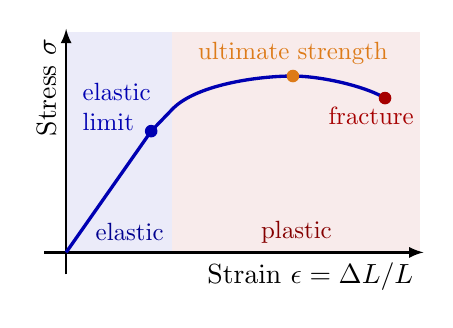
\begin{tikzpicture}
  \def\xmax{4.5}
  \def\ymax{2.8}
  \def\xa{0.24*\xmax} % elastic limit
  \def\xb{0.30*\xmax} % yield strength
  \def\xc{0.64*\xmax} % ultimate strength
  \def\xd{0.90*\xmax} % facture
  \coordinate (O) at (0,0); % origin
  \coordinate (A) at (\xa,0.55*\ymax); % elastic limit
  \coordinate (B) at (\xb,0.65*\ymax); % yield strength
  \coordinate (C) at (\xc,0.80*\ymax); % ultimate strength
  \coordinate (D) at (\xd,0.70*\ymax); % facture
  \fill[myblue!8] (0,0) rectangle (\xb,\ymax);
  %\fill[myorange!10] (\xa,0) rectangle (\xb,\ymax);
  \fill[myred!8] (\xb,0) rectangle (\xmax,\ymax);
  \draw[->,thick] (-0.1*\ymax,0) -- (0.04+\xmax,0) node[below left=0] {Strain $\epsilon=\Delta L/L$};
  \draw[->,thick] (0,-0.1*\ymax) -- (0,0.04+\ymax) node[above left=0,rotate=90] {Stress $\sigma$};
  %\draw[thick] ({(\xa+\xb)/2},0.035*\ymax) --++ (0,-0.07*\ymax);
  \draw[myblue,very thick]
    (O) -- (A) -- (B) to[out=46,in=180,looseness=0.7] (C) to[out=0,in=150,looseness=0.7]  (D);
  \fill[myblue] (A) circle(0.08) node[above left=-3,scale=0.9,align=left] {elastic\\limit};
  \fill[myorange] (C) circle(0.08) node[above=1,scale=0.9] {ultimate strength};
  \fill[myred] (D) circle(0.08) node[left=5,below,scale=0.9] {fracture};
  \node[right=1,above left=1,myblue!80!black,scale=0.9] at (\xb,0) {elastic};
  \node[above,myred!80!black,scale=0.9] at ({(\xmax+\xb)/2},0) {plastic};
\end{tikzpicture}


\end{document}
